\documentclass{article}
\usepackage{graphicx} % Required for inserting images
\usepackage{enumitem}
\usepackage{enumerate}
\usepackage{gensymb}
\usepackage[margin=1in]{geometry}
\title{Introduction to Forces}


\date{}
\begin{document}

\maketitle

\section{Initial thoughts and motivation}
\subsection{Where are we now?}
In our previous section we laid the groundwork for our study of physics, saying that we wished - as the first physicists in the Universe - to understand the world around us. 

We embarked on this endeavour by starting to point out things that we observe, and in the process of doing so we realized that space does not look the same to everyone, and observations of the Universe will depend on who is observing. In terms of physics, this insight of relativity - \textit{Galilean relativity} to be precise - is quite profound, that the Universe does not look the same to every observer. In the context of olympiads - which we are particularly interested in - we saw that this insight led to a particularly clever technique: whenever we are faced with a problem we can choose to view the system from the observer (frame of reference) according to which the system looks the simplest. This often makes a problem vastly simpler, and sometimes trivializes it completely. Finding which reference frame is the "simplest" is the tricky part of this technique, and there is no simple recipe for finding the best frame. Nevertheless - as is typical in problem solving - we learned that there are some guidelines ("heuristics") one can follow in trying to find these simple frames. 
   
The better you get at finding these frames, the better problem solver you will become. For the purpose of all problems moving forward, I encourage you to always consider which frame you think would be the best to view this system in. Thereafter, please proceed with your calculations. For instance, if a system consists of only two objects but they are both moving, you may want to start by considering the system in the frame of one of the objects, such that there is only one moving part.

%\subsection{Origins of physics}
%When we first started observing the world, we wanted to find some answers to the underlying structure of the Universe (answering questions like "how do things move" and "why do things happen") but we got so caught up discussing how the Universe looks different for different observers that we actually did not make any progress on this first question. Now that we have slightly more formally established the notion of \textit{what} we observe - by introducing the idea of reference frames - we can now dig into the question of how the Universe actually works.

%So, maybe we start by asking a very simple, very fundamental question: why does something happen in the Universe, as opposed to not happening? This is a wonderful question, but it is so broad that we can't quite make progress on it. We may be better off focusing on a particular type of events, and understand why they happen as opposed to not happening. In fact, it seems that this is much the reason why we have different (theoretical) academic subjects now: they are all focused on answering this question, but regarding different kinds of events. Physics may be seen as one of the more fundamental of these subjects, since it concerns - probably - one of the first obvious kinds of events: motion of non-living things. 

%Inherently, the fact that things which appear to be non-living actually move around (such as waves rolling in the sea or rain falling from the sky) and do things is quite peculiar. As far as we know, these things have no agency on their own, so they are not themselves choosing to move in the way they do. So, that begs the question, what causes these things to move in the way they do? Is there an underlying structure behind the way they move or is it just random? These are the very fundamental questions which physics seeks to answer.

%\subsection{Fundamentals of mechanics}
%This question (why do seemingly non-living things act the way they do?) is essentially what Newton was asking himself - albeit it in a specific form - when he first pondered why an apple falls from a tree. Are there any underlying laws which govern the motion of all objects (also called bodies) in the Universe? If so, what are they? Newton started with this very simple - but also very profound - question, and what he came up with from observation is what we today call Newton's Laws of Mechanics. Together, these form the system of Newtonian Mechanics, which is the first full system for understanding physical events. We shall see later - as physicists found out in the late 19th century - that this system is incomplete - or rather, not quite correct - but it is amazingly accurate in many cases, particularly most of those we see with our own eyes.

%We shall consider this system in some detail. It is amazingly simple - considering the complexity of the world which it describes - and before we delve into it I encourage you to put yourself in the shoes of Isaac Newton, before any full system describing the Universe had been put in place. Considering the vast variety of different things you can see in the world, do you have any idea of how complex the laws governing it must be? This is the beauty of Newtonian mechanics: our complex Universe seems to be at its core (mostly) governed by very simple rules.
   
%Note that Newtonian mechanics is not the only formulation of classical mechanics! In fact, many things make more sense in the system proposed by Lagrange or Hamilton (see Landau \& Lifschitz for more).

\subsection{Newtonian mechanics}
Now, having dealt with the question of accurately describing \textit{what} is happening in the Universe, we get into the question of \textit{why} or \textit{how} things are happening. The very first attempt at formalizing observations into a complete system which can describe events in the Universe was made by Newton. I will assume here that you are familiar with Newton's laws from before, and will just simply state them here:

\begin{enumerate}[I.]
    \item A body remains at rest or moving with constant velocity, if and only if there is no net force acting on it.
    \item The net force on a body equals the body's acceleration times its mass ($F=ma$)
    \item If one body exerts a force on a second body, then that second body always exerts a force equal in magnitude but opposite in direction on the first body. 
\end{enumerate}

You will likely have seen these before in your high school physics course, and so I will not delve into the details of them here, and instead I hope much of their nuances will gradually become clearer as we do more problems with these. Nevertheless, it is worth taking a step back and just admiring the simplicity of these laws, given the complexity of the physical phenomena that we still observe within mechanics.

Also, Newton's laws are centred around the idea of the \textit{\textbf{force}}. This is the fundamental core of his mechanical system. \textbf{Forces are vectors}, and as such we can sometimes solved problems just using the vectors in free space, which is a very nice property. Other than that however, the physical intuition behind forces is  quite opaque (at least to me), and I think we are yet to find a really good intuition for what they are. You may consider it left as an exercise for the reader.

But, with Newton's laws in hand we are ready to start solving a whole host of mechanics problems. First, I will just briefly outline some typical forces that we come across in these problems.

\subsection{Examples of forces}
\subsubsection{Gravity}
In Newtonian mechanics, gravitational forces follow Newton "Universal" Law of Gravity. For simpler scenarios, such as those on Earth, we may consider the gravitational field to always be constant, hence:
\[\boldsymbol{F} = m \boldsymbol{g}\]

Bold here symbolizes that something is a vector. On Earth, $\boldsymbol{g}$ is $~9.8 m s^{-1}$ in the negative vertical direction (note that this is a vector).

\subsubsection{Normal force}
Normal force is just the force between two objects which are in contact with each other. Importantly, this forces is \textit{always} perpendicular to the surfaces of the two objects at the point of contact. ¨

\subsubsection{Friction force}
The friction force arises due to the "rubbing" of rough surface against each other. Importantly, the firction force is proportional to the normal force between the objects. Hence we can write for friction for $F_d$

\[F_d = \mu N\]

where $\mu$ is the \textit{coefficient of friction}.

\subsubsection{Tension force}
This is the force which works internally in something like a rope or a string, and which keeps it together. Tension is a tricky one to figure out (at least has been for me). I advise proceeding with caution and carefully applying Newton's laws rigorously when trying to find tension forces. I attached some questions below to get you to think about some non-intuitive facts about tension forces.

\section{Questions}

\subsection{Check your understanding}
\begin{enumerate}

\item Two people pull on opposite ends of a rope, each with a force F. What is the tension in the rope?

\item Two teams, Brann and Viking, are competing in a tug-of-war. Brann pulls at the rope with a force of $5000 N$, but Viking is currently winning (the rope is moving towards their end). Which of the following statements is correct? 
    \begin{enumerate}[A.]
        \item Viking is pulling at the rope with a force greater than $5000$ N.
        \item Viking is pulling at the rope with a force of $5000$ N.
    \end{enumerate}

\item A mass $m$ rests on an incline with angle $\alpha$ (like in figure \ref{mass sliding down incline}. What must the coefficient of friction be to stop the block from sliding down?

\item You're hopping upwards and forwards. Which of the figures in figure \ref{forces in jump} most accurately shows the forces working on you?
\end{enumerate}

\begin{figure}
    \centering
    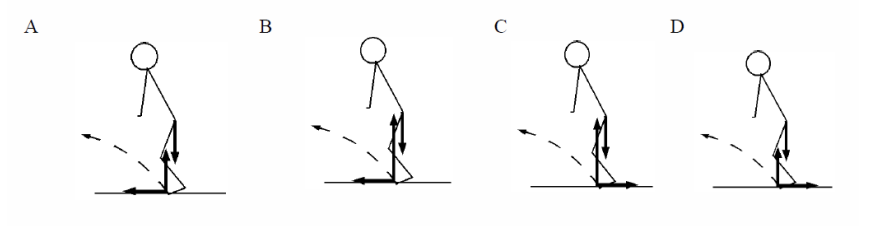
\includegraphics[width=0.5\linewidth]{assets/jumps.png}
    \caption{Forces in jump}
    \label{forces in jump}
\end{figure}

\begin{figure}
    \centering
    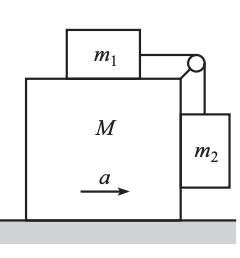
\includegraphics[width=0.5\linewidth]{assets/masses on mass.png}
    \caption{Masses on mass}
    \label{masses on mass}
\end{figure}

\subsection{Trying out the waters}

\begin{enumerate}

\item All of the surfaces in the setup in figure \ref{masses on mass} are frictionless. You push on the large block and give it an acceleration $\alpha$. For what value of $\alpha$ is there no relative motion among the masses?

\item In Figure \ref{box with force}, if the box is stationary and the angle u between the horizontal and force is increased
\begin{figure}
    \centering
    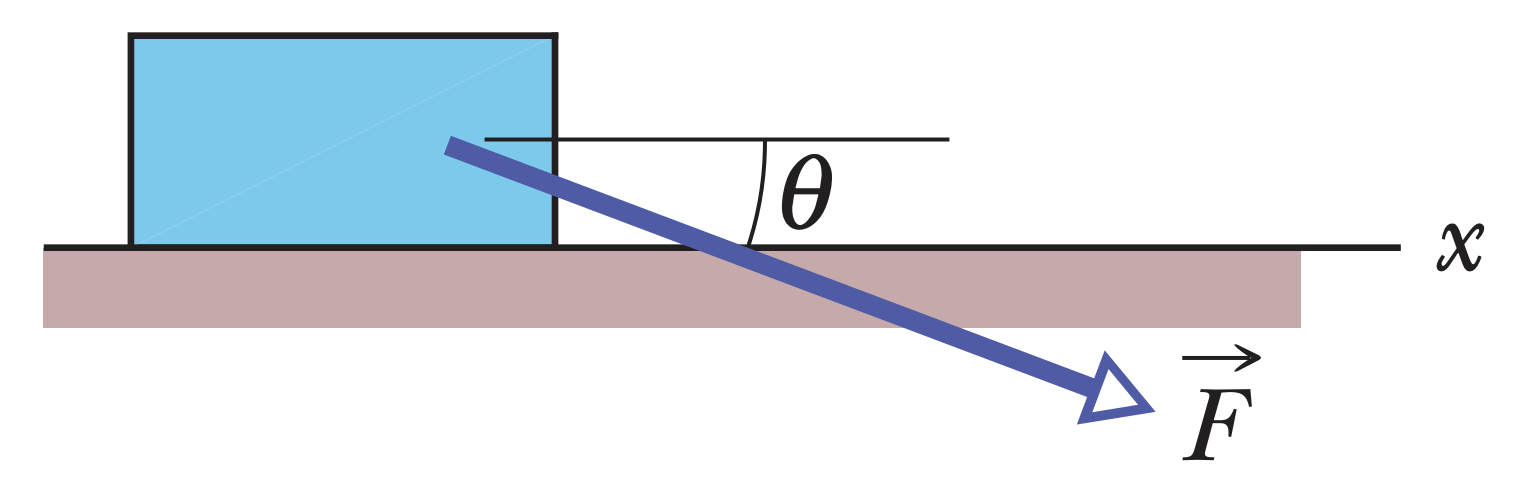
\includegraphics[width=0.5\linewidth]{box with force.png}
    \caption{Box with force}
    \label{box with force}
\end{figure}
somewhat, do the following quantities increase, decrease, or remain the
same: (a) $F_x$ (horizontal force); (b) $f_s$ (frcition force); (c) $F_N$ (normal force)?

\item A small body $A$ starts sliding down from the top of a wedge whose base is equal to $l = 2.10 m$. The coefficient of friction between the body and the wedge is $k = 0.140$. At what value of the angle $\alpha$ will the time of sliding be the least. What will it be equal to?

\item A block of mass $M_1$ sits on a block of mass $M_2$ on a frictionless table. The
coefficient of friction between the blocks is $\mu$. Find the maximum horizontal force that can be
applied to (a) block 1 or (b) block 2 so that the blocks will not slip on each other.

\item A small body was launched up an inclined planeset at an angle $\alpha = 15 \degree$ against the horizontal. Find the coefficient of friction, if the time of the ascent of the body is $\eta = 2.0$ times less than the time of its decent. 

\item The inclined plane of figure \ref{masses with pulley on incline} forms an angle $\alpha = 30 \degree$ with the horizontal. The mass ratio $m_1/m_2 = \eta$ = 2/3{. The coefficient of friction between the body $m_1$ and the inclined plane $k = 0.10$. The masses of the pulley and the threads are negligible. Find the magnitude and the direction of acceleration of the body $m_2$ when the formerly stationary system starts moving. 


\end{enumerate}
\begin{figure}
    \centering
    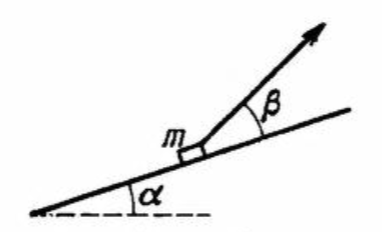
\includegraphics[width=0.5\linewidth]{assets/mass on incline.png}
    \caption{Mass pulled up on incline}
    \label{mass pulled up incline}
\end{figure}

\begin{figure}
    \centering
    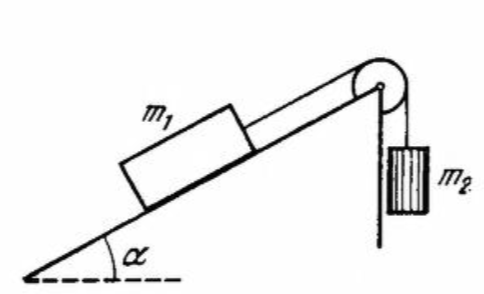
\includegraphics[width=0.5\linewidth]{assets/masses with pulley on incline.png}
    \caption{Masses with pulley on incline}
    \label{masses with pulley on incline}
\end{figure}



\begin{figure}
    \centering
    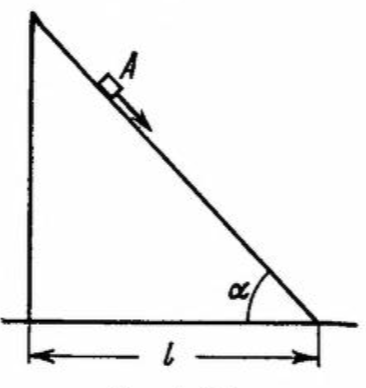
\includegraphics[width=0.5\linewidth]{assets/masses sliding down incline.png}
    \caption{Mass sliding down incline}
    \label{mass sliding down incline}
\end{figure}

\subsection{Olympiad style questions}
\begin{enumerate}
\item A small object is at rest on the edge of a horizontal table. It is pushed in such a way that it falls off the other side of the table, which is 1m wide, after 2 s. Does the object have wheels?

\item A ball is dropped from rest at height $4h$. After it has fallen a distance $d$, a second ball is
dropped from rest at height $h$. What should $d$ be (in terms of $h$) so that the balls hit the
ground at the same time?

\item $N$ identical uniform bricks of length L are stacked, one above the other, near the edge
of a table. What is the maximum possible length the top brick can protrude over the edge of the
table? How does this limit grow as $N$ goes to infinity?

\item A bar of mass $m$ is pull up by means of a thread up an inclined plane forming an angle $\alpha$ with the horizontal (see figure \ref{mass pulled up incline}). The coefficient of friction is equal to $k$. Find the angle $\beta$ which the thread must form with the inclined plane for the tension of the thread to be minimum. What is it equal to?
\end{enumerate}

\end{document}




